\documentclass{article}\usepackage[]{graphicx}\usepackage[]{xcolor}
% maxwidth is the original width if it is less than linewidth
% otherwise use linewidth (to make sure the graphics do not exceed the margin)
\makeatletter
\def\maxwidth{ %
  \ifdim\Gin@nat@width>\linewidth
    \linewidth
  \else
    \Gin@nat@width
  \fi
}
\makeatother

\definecolor{fgcolor}{rgb}{0.345, 0.345, 0.345}
\newcommand{\hlnum}[1]{\textcolor[rgb]{0.686,0.059,0.569}{#1}}%
\newcommand{\hlsng}[1]{\textcolor[rgb]{0.192,0.494,0.8}{#1}}%
\newcommand{\hlcom}[1]{\textcolor[rgb]{0.678,0.584,0.686}{\textit{#1}}}%
\newcommand{\hlopt}[1]{\textcolor[rgb]{0,0,0}{#1}}%
\newcommand{\hldef}[1]{\textcolor[rgb]{0.345,0.345,0.345}{#1}}%
\newcommand{\hlkwa}[1]{\textcolor[rgb]{0.161,0.373,0.58}{\textbf{#1}}}%
\newcommand{\hlkwb}[1]{\textcolor[rgb]{0.69,0.353,0.396}{#1}}%
\newcommand{\hlkwc}[1]{\textcolor[rgb]{0.333,0.667,0.333}{#1}}%
\newcommand{\hlkwd}[1]{\textcolor[rgb]{0.737,0.353,0.396}{\textbf{#1}}}%
\let\hlipl\hlkwb

\usepackage{framed}
\makeatletter
\newenvironment{kframe}{%
 \def\at@end@of@kframe{}%
 \ifinner\ifhmode%
  \def\at@end@of@kframe{\end{minipage}}%
  \begin{minipage}{\columnwidth}%
 \fi\fi%
 \def\FrameCommand##1{\hskip\@totalleftmargin \hskip-\fboxsep
 \colorbox{shadecolor}{##1}\hskip-\fboxsep
     % There is no \\@totalrightmargin, so:
     \hskip-\linewidth \hskip-\@totalleftmargin \hskip\columnwidth}%
 \MakeFramed {\advance\hsize-\width
   \@totalleftmargin\z@ \linewidth\hsize
   \@setminipage}}%
 {\par\unskip\endMakeFramed%
 \at@end@of@kframe}
\makeatother

\definecolor{shadecolor}{rgb}{.97, .97, .97}
\definecolor{messagecolor}{rgb}{0, 0, 0}
\definecolor{warningcolor}{rgb}{1, 0, 1}
\definecolor{errorcolor}{rgb}{1, 0, 0}
\newenvironment{knitrout}{}{} % an empty environment to be redefined in TeX

\usepackage{alltt}
\usepackage{amsmath} %This allows me to use the align functionality.
                     %If you find yourself trying to replicate
                     %something you found online, ensure you're
                     %loading the necessary packages!
\usepackage{amsfonts}%Math font
\usepackage{graphicx}%For including graphics
\usepackage{hyperref}%For Hyperlinks
\usepackage[shortlabels]{enumitem}% For enumerated lists with labels specified
                                  % We had to run tlmgr_install("enumitem") in R
\hypersetup{colorlinks = true,citecolor=black} %set citations to have black (not green) color
\usepackage{natbib}        %For the bibliography
\setlength{\bibsep}{0pt plus 0.3ex}
\bibliographystyle{apalike}%For the bibliography
\usepackage[margin=0.50in]{geometry}
\usepackage{float}
\usepackage{multicol}

%fix for figures
\usepackage{caption}
\newenvironment{Figure}
  {\par\medskip\noindent\minipage{\linewidth}}
  {\endminipage\par\medskip}
\IfFileExists{upquote.sty}{\usepackage{upquote}}{}
\begin{document}
\title{Lab 7-8 -- MATH 240 -- Computational Statistics}

\author{
  Jackson Colby \\
  Colgate University  \\
  Mathematics  \\
  {\tt jcolby@colgate.edu}
}

\date{}

\maketitle

\begin{multicols}{2}

\section{Introduction}

\section{Density Functions and Parameters}

The Beta distribution with parameters \( \alpha \) and \( \beta \) is given by the probability density function:

\[
f_X(x | \alpha, \beta) = \frac{\Gamma(\alpha + \beta)}{\Gamma(\alpha) \Gamma(\beta)} x^{\alpha - 1} (1 - x)^{\beta - 1}, \quad \text{for } x \in [0, 1]
\]

The probability function for the Beta distribution takes values of 0 everywhere outside of [0,1]. 


The following plot shows the comparison between a Beta distribution with \(\alpha=5\) and \(\beta=5\) and a Gaussian distribution with the same mean and variance. This figure shows that when alpha and beta are the same or close to the same the beta distribution has a similar density to the normal distribution. If \(\alpha\) is greater than \(\beta\) then the distribution will be left skewed and if \(\alpha\) is less than \(\beta\) then the distribution will be right skewed. 

\begin{knitrout}
\definecolor{shadecolor}{rgb}{0.969, 0.969, 0.969}\color{fgcolor}
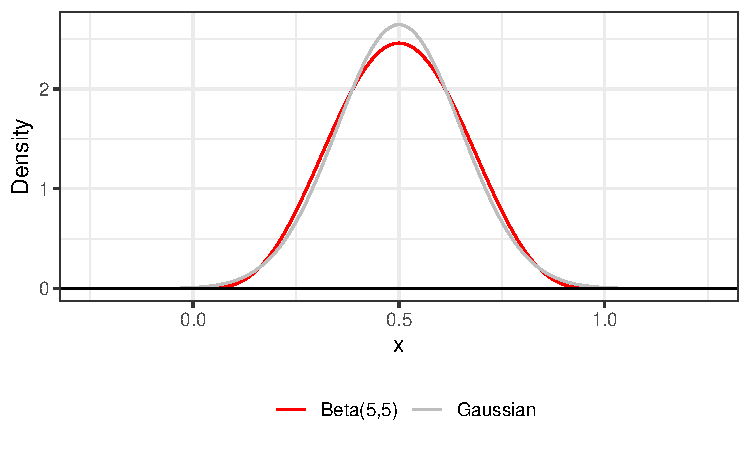
\includegraphics[width=\maxwidth]{figure/unnamed-chunk-1-1} 
\end{knitrout}

A table containing the four given cases is below.


% latex table generated in R 4.4.2 by xtable 1.8-4 package
% Tue Apr  1 00:01:17 2025
\begin{table}[H]
\centering
\begingroup\small
\begin{tabular}{rrrrrr}
  \hline
alpha & beta & mean & variance & skewness & kurtosis \\ 
  \hline
2.00 & 5.00 & 0.29 & 0.03 & 0.60 & -0.12 \\ 
  5.00 & 5.00 & 0.50 & 0.02 & 0.00 & -0.46 \\ 
  5.00 & 2.00 & 0.71 & 0.03 & -0.60 & -0.12 \\ 
  0.50 & 0.50 & 0.50 & 0.12 & 0.00 & -1.50 \\ 
   \hline
\end{tabular}
\endgroup
\caption{Summary of Beta Distribution Statistics} 
\end{table}

As seen in the table, for larger \(\alpha\) and \(\beta\) the variance is lower. All the Beta distributions are platykurtic, the graphs being more platykurtic when \(\alpha\) and \(\beta\) are the same or similar. 

\section{Properties}
The population level properties for the Beta Distribution are as follows:
The mean is given by:
\[
E(X) = \frac{\alpha}{\alpha + \beta}
\]
The variance is given by:
\[
\text{Var}(X) = \frac{\alpha \beta}{(\alpha + \beta)^2 (\alpha + \beta + 1)}
\]
The skewness is given by:
\[
\text{Skew}(X) = \frac{2(\beta - \alpha)}{(\alpha + \beta + 1)\sqrt{(\alpha + \beta + 2)\alpha \beta}}
\]
The excess kurtosis is given by:
\[
\text{Kurt}(X) = \frac{6(\alpha - \beta)^2}{(\alpha + \beta + 1)\left(\alpha + \beta + 2\right)} - \frac{\alpha \beta (\alpha + \beta + 2)}{\alpha \beta (\alpha + \beta + 2)(\alpha + \beta + 3)}
\]

A function called beta.moment was utilized to test both centered and uncentered moments of the population-level characteristics to the approximations calculated. 

For the case alpha=2, beta=5: the statistics using the population level were mean=0.285714, var=0.0255102, skew=0.047619, kurt=0.001874.
These statistics compared to the table above are very close to the values of the approximation, meaning the characteristics described above are true for the Beta Distribution.

\section{Estimators}
For the case where alpha=2 and beta=5, the following summary statistics were calculated for a sample of 500.



% latex table generated in R 4.4.2 by xtable 1.8-4 package
% Tue Apr  1 00:01:17 2025
\begin{table}[H]
\centering
\begingroup\small
\begin{tabular}{rrrr}
  \hline
mean\_sample & variance\_sample & skewness\_sample & kurtosis\_sample \\ 
  \hline
0.29 & 0.03 & 0.57 & -0.23 \\ 
   \hline
\end{tabular}
\endgroup
\caption{Summary Statistics for Beta Sample} 
\end{table}


Below is a distribution showing the estimated density and the actual Beta Distribtuion over the sample.
\begin{knitrout}
\definecolor{shadecolor}{rgb}{0.969, 0.969, 0.969}\color{fgcolor}
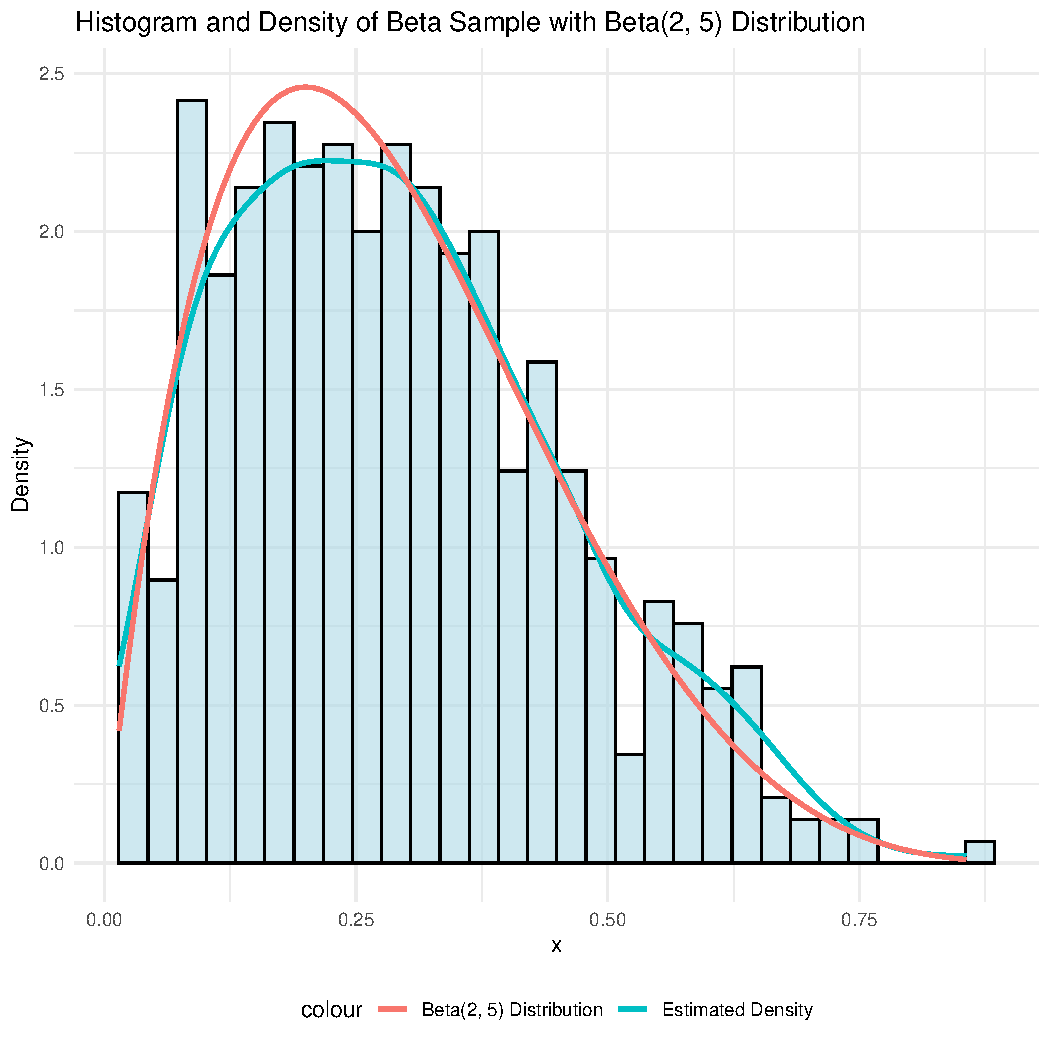
\includegraphics[width=0.4\textwidth,height=0.2\textheight]{figure/plot_beta_sample-1} 
\end{knitrout}

As seen in the plot, the estimated density does a good job of fitting the data, and fits similarly compared to the actual Beta(2,5) Distribution.

Utilizing the packages cumstats \citep{cumstats} and patchwork \citep{patchwork}, we created plots that tracked the path of the summary statistics for different samples as n goes to 500.
\begin{knitrout}
\definecolor{shadecolor}{rgb}{0.969, 0.969, 0.969}\color{fgcolor}
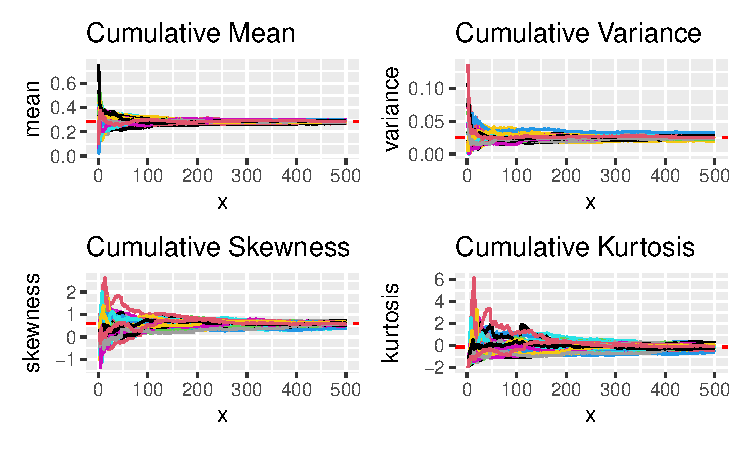
\includegraphics[width=\maxwidth]{figure/unnamed-chunk-5-1} 
\end{knitrout}

As seen in the plot above, as n (the sample size), gets larger all the samples converge to the same values meaning that any random sample is sufficient for calculating the mean, variance, etc.  of the Beta Distribution, and the sample size is important because the larger sample size leads to a better approximation.

The variation of the mean, variance, etc. can be shown in the plots below in the Appendix.
All four of the plots follow close to normal distributions, showing that the samples of all mean, variance, etc. follow close to a Gaussian distribution, forming a bell shaped curve.

\section{Example with Death Rates Data}




\begin{tiny}
\bibliography{bib}
\end{tiny}
\end{multicols}

\newpage

\section{Appendix}
\subsection{Estimators}
\begin{knitrout}
\definecolor{shadecolor}{rgb}{0.969, 0.969, 0.969}\color{fgcolor}
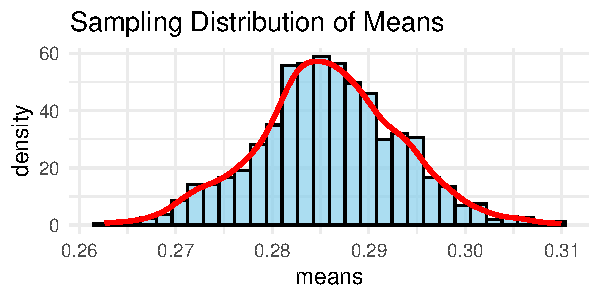
\includegraphics[width=\maxwidth]{figure/unnamed-chunk-6-1} 
\end{knitrout}

\begin{knitrout}
\definecolor{shadecolor}{rgb}{0.969, 0.969, 0.969}\color{fgcolor}
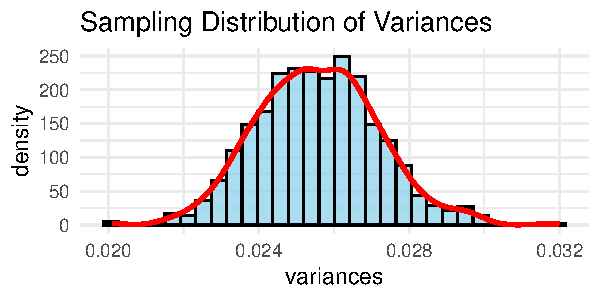
\includegraphics[width=\maxwidth]{figure/unnamed-chunk-7-1} 
\end{knitrout}

\begin{knitrout}
\definecolor{shadecolor}{rgb}{0.969, 0.969, 0.969}\color{fgcolor}
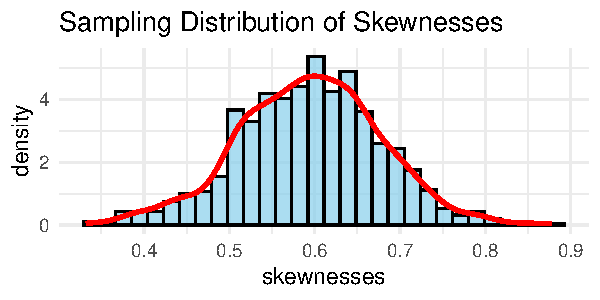
\includegraphics[width=\maxwidth]{figure/unnamed-chunk-8-1} 
\end{knitrout}

\begin{knitrout}
\definecolor{shadecolor}{rgb}{0.969, 0.969, 0.969}\color{fgcolor}
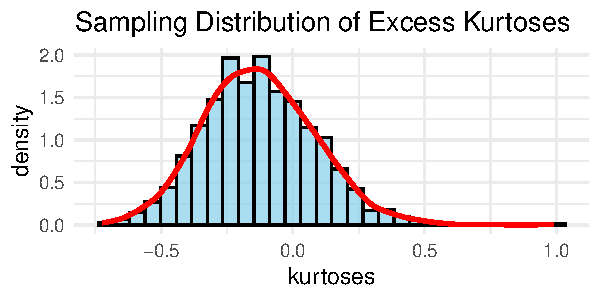
\includegraphics[width=\maxwidth]{figure/unnamed-chunk-9-1} 
\end{knitrout}


\end{document}
